\documentclass[tikz, border=4pt]{standalone}
% Shared preamble for the qpo_*.tex query plan figures.
\usepackage[T1]{fontenc}
\usepackage{lmodern}
\usetikzlibrary{arrows.meta, positioning, fit, backgrounds, calc}

\definecolor{accent}{HTML}{2F5D8C}
\definecolor{groupfill}{HTML}{EEF3F8}
\definecolor{taskfill}{HTML}{FFFFFF}
\definecolor{note}{HTML}{555555}
\definecolor{hot}{HTML}{C0561B}
\definecolor{hotfill}{HTML}{FCEBDD}

\newcommand{\sub}{\tiny\color{note}}
\newcommand{\hsub}{\tiny\color{hot}}

\tikzset{
    every picture/.style={font=\sffamily\scriptsize, node distance=4mm},
    op/.style={draw=accent, fill=taskfill, rounded corners=2pt, line width=0.6pt,
               minimum width=30mm, minimum height=7mm, align=center, inner sep=2pt},
    tbl/.style={op, fill=groupfill},
    small/.style={minimum width=18mm},
    hot/.style={draw=hot, fill=hotfill, line width=1pt},
    flow/.style={-{Stealth[length=2mm]}, accent, line width=0.7pt},
    hotflow/.style={flow, color=hot, line width=0.9pt},
    panel/.style={draw=accent, dashed, rounded corners=4pt, line width=0.6pt, inner sep=3mm},
    lbl/.style={font=\sffamily\scriptsize\bfseries, text=accent},
    callout/.style={font=\sffamily\tiny, text=hot, align=left},
}

\begin{document}
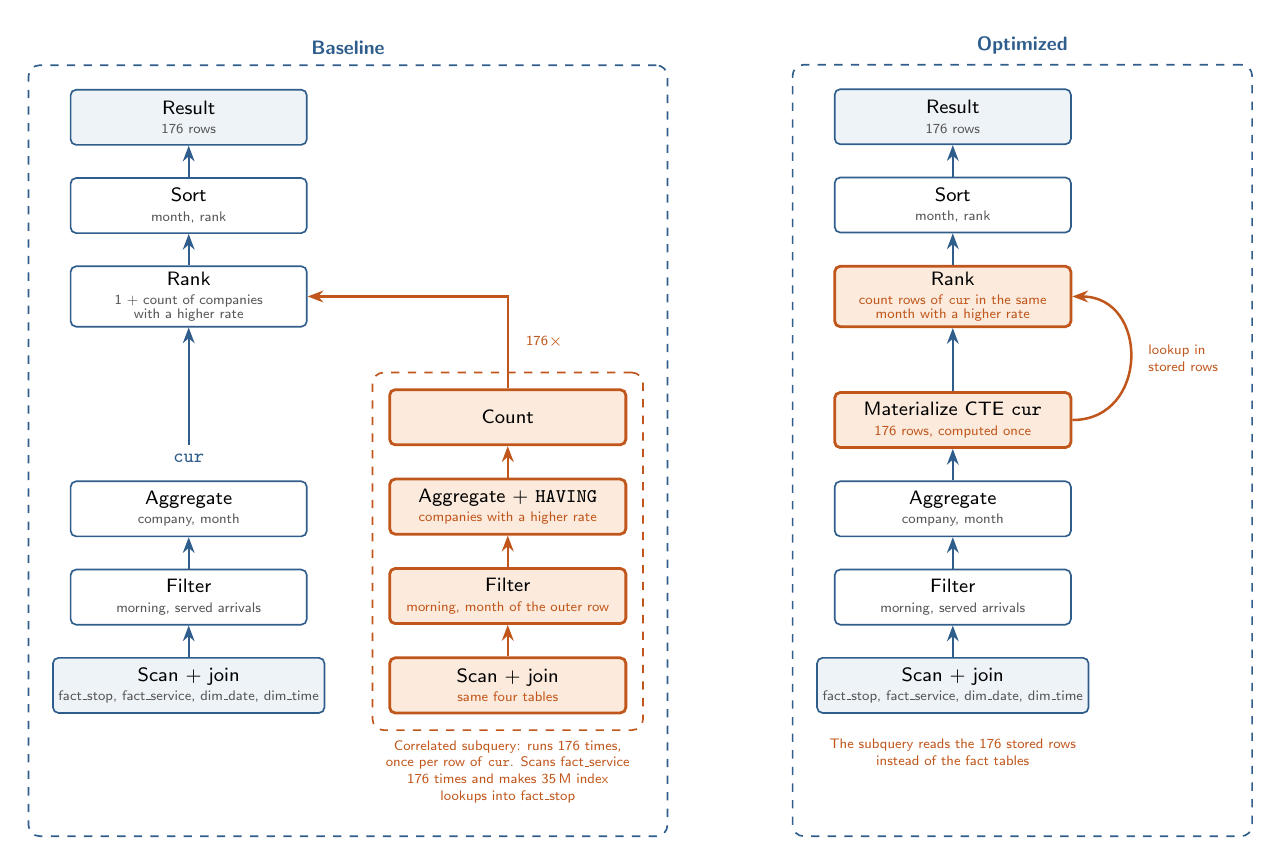
\begin{tikzpicture}

% ---------------- Baseline: main branch ----------------
\node[tbl] (bs) {Scan + join\\[-1pt]{\sub fact\_stop, fact\_service, dim\_date, dim\_time}};
\node[op, above=of bs] (bf) {Filter\\[-1pt]{\sub morning, served arrivals}};
\node[op, above=of bf] (ba) {Aggregate\\[-1pt]{\sub company, month}};
\node[lbl, above=1mm of ba] (bc) {\texttt{cur}};

\draw[flow] (bs) -- (bf);
\draw[flow] (bf) -- (ba);

% ---------------- Baseline: correlated subquery ----------------
\node[tbl, hot, right=8mm of bs] (ss) {Scan + join\\[-1pt]{\hsub same four tables}};
\node[op, hot, above=of ss] (sf) {Filter\\[-1pt]{\hsub morning, month of the outer row}};
\node[op, hot, above=of sf] (sa) {Aggregate + \texttt{HAVING}\\[-1pt]{\hsub companies with a higher rate}};
\node[op, hot, above=of sa] (sc) {Count};

\draw[hotflow] (ss) -- (sf);
\draw[hotflow] (sf) -- (sa);
\draw[hotflow] (sa) -- (sc);

\begin{scope}[on background layer]
  \node[panel, draw=hot, fit=(ss)(sc), inner sep=2mm] (sub) {};
\end{scope}
\node[callout, anchor=north, align=center] (snote) at (sub.south) {Correlated subquery: runs 176 times,\\once per row of \texttt{cur}. Scans fact\_service\\176 times and makes 35\,M index\\lookups into fact\_stop};

% ---------------- Optimized ----------------
\node[tbl, right=24mm of ss] (os) {Scan + join\\[-1pt]{\sub fact\_stop, fact\_service, dim\_date, dim\_time}};
\node[op, above=of os] (of) {Filter\\[-1pt]{\sub morning, served arrivals}};
\node[op, above=of of] (oa) {Aggregate\\[-1pt]{\sub company, month}};
\node[op, hot, above=of oa] (om) {Materialize CTE \texttt{cur}\\[-1pt]{\hsub 176 rows, computed once}};
\node[op, hot, above=8mm of om] (ork) {Rank\\[-1pt]{\hsub count rows of \texttt{cur} in the same}\\[-3pt]{\hsub month with a higher rate}};
\node[op, above=of ork] (oo) {Sort\\[-1pt]{\sub month, rank}};
\node[op, fill=groupfill, above=of oo] (or) {Result\\[-1pt]{\sub 176 rows}};

\draw[flow] (os) -- (of);
\draw[flow] (of) -- (oa);
\draw[flow] (oa) -- (om);
\draw[flow] (om) -- (ork);
\draw[hotflow] (om.east) to[out=0, in=0, looseness=1.6]
    node[callout, right=1mm, align=left] (lk) {lookup in\\stored rows} (ork.east);
\draw[flow] (ork) -- (oo);
\draw[flow] (oo) -- (or);

\node[callout, below=2mm of os, align=center] (onote)
    {The subquery reads the 176 stored rows\\instead of the fact tables};

\begin{scope}[on background layer]
  \node[panel, fit=(os)(or)(onote)(lk)(snote.south -| os)] (opp) {};
\end{scope}
\node[lbl, anchor=south] at (opp.north) {Optimized};

% ---------------- Baseline top, aligned with the optimized side ----------------
\node[op] (brk) at (ba |- ork) {Rank\\[-1pt]{\sub 1 + count of companies}\\[-3pt]{\sub with a higher rate}};
\node[op, above=of brk] (bo) {Sort\\[-1pt]{\sub month, rank}};
\node[op, fill=groupfill, above=of bo] (br) {Result\\[-1pt]{\sub 176 rows}};

\draw[flow] (bc.north) -- (brk);
\draw[hotflow] (sc.north) |- node[callout, pos=0.25, right=1mm] {176$\times$} (brk.east);
\draw[flow] (brk) -- (bo);
\draw[flow] (bo) -- (br);

\begin{scope}[on background layer]
  \node[panel, fit=(bs)(br)(sub)(snote)] (bp) {};
\end{scope}
\node[lbl, anchor=south] at (bp.north) {Baseline};

\end{tikzpicture}
\end{document}
